% \Image{Capa do livro (; )}{PNLD2022-004-01.png}
% \Image{Ilustração do livro (Ayllon/Fábio Zimbres; Ayllon)}{PNLD2022-004-04.png}
% \Image{Ilustração do livro (Ayllon/Fábio Zimbres; Ayllon)}{PNLD2022-004-05.png}
% \Image{Ilustração do livro (Ayllon/Fábio Zimbres; Ayllon)}{PNLD2022-004-06.png}


\documentclass[11pt]{extarticle}
\usepackage{manualdoprofessor}
\usepackage{fichatecnica}
\usepackage{lipsum,media9}
\usepackage[justification=raggedright]{caption}
\usepackage[one]{bncc}
\usepackage[ayllon]{../edlab}
\usepackage{marginnote}
\usepackage{pdfpages}
\usepackage[printwatermark]{xwatermark}
%\newwatermark[pagex=2]{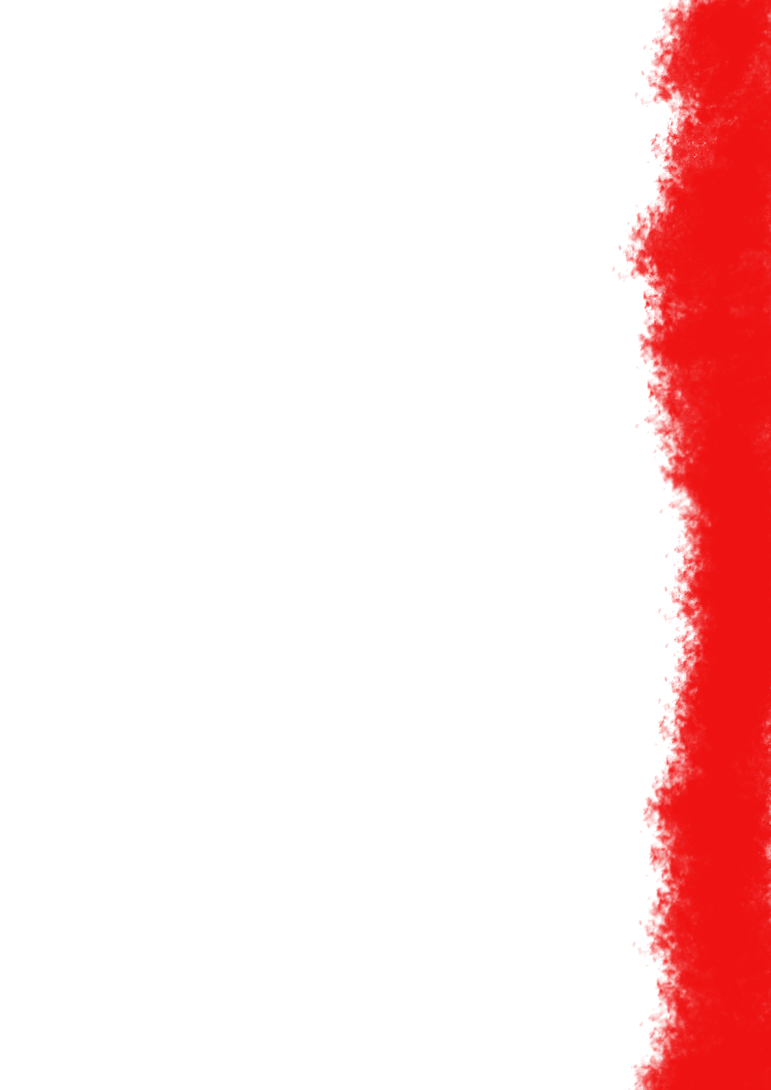
\includegraphics[scale=3.3]{watermarks/test-a.png}}	% página específica
%\newwatermark[oddpages]{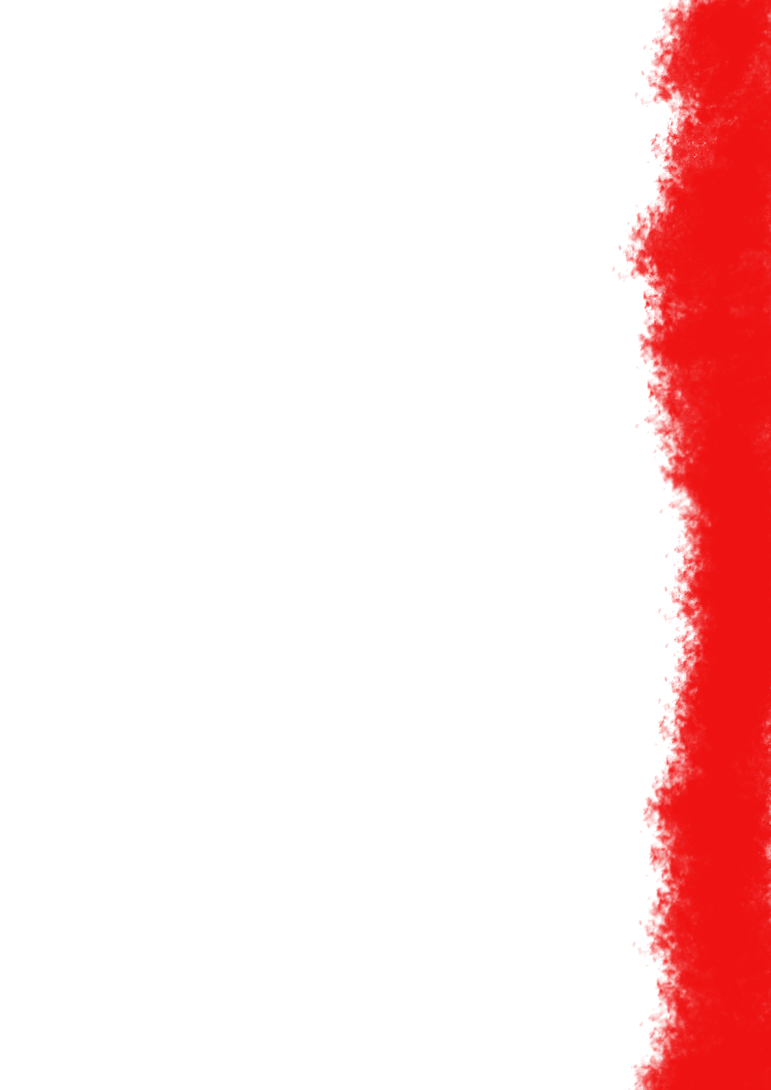
\includegraphics{watermarks/test-a.png}}			% páginas ímpars
%\newwatermark[evenpages]{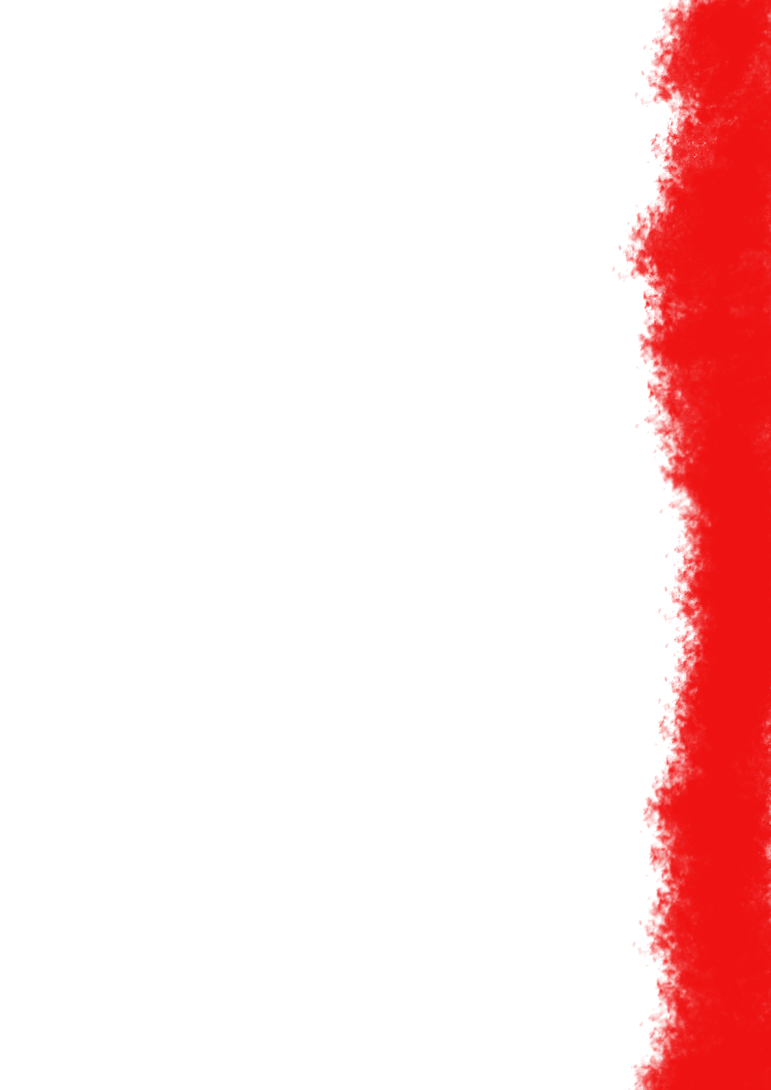
\includegraphics{watermarks/test-a.png}}			% págimas pares
\newwatermark[allpages]{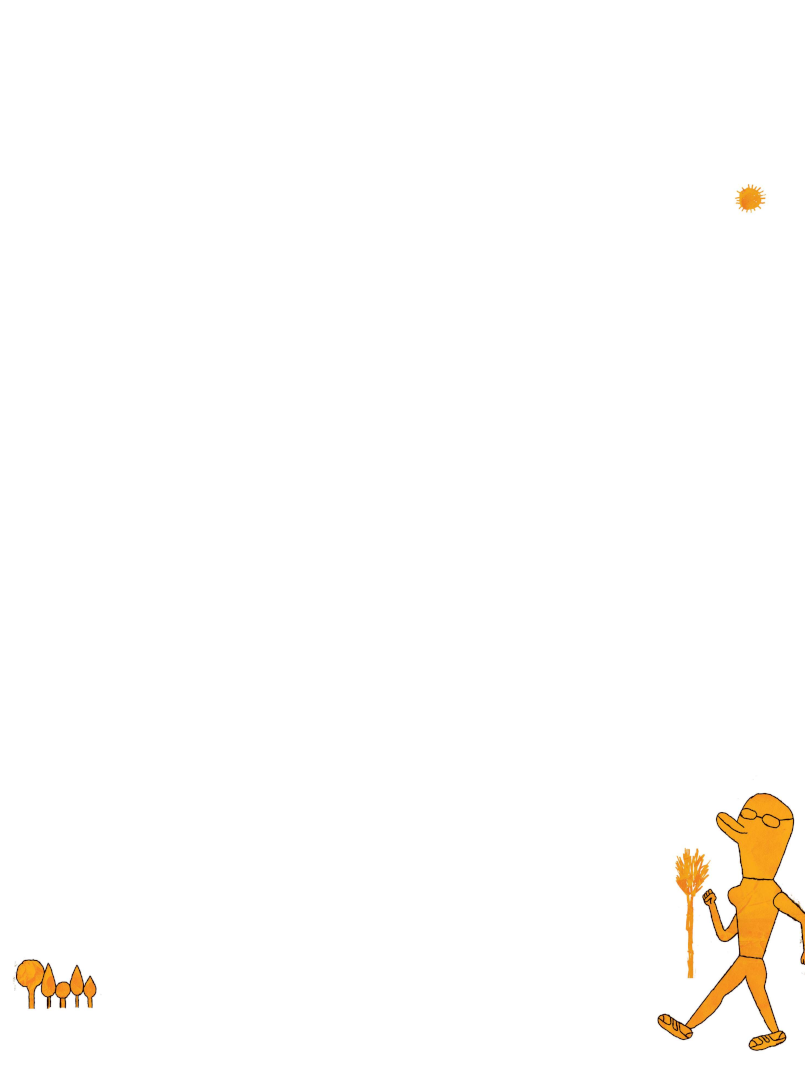
\includegraphics[scale=1]{watermarks/004.png}}

%\pagecolor{cyan!0!magenta!10!yellow!28!black!28!}

\newcommand{\AutorLivro}{Fábio Zimbres}
\newcommand{\TituloLivro}{Cada qual com seu gosto}
\newcommand{\Tema}{Relacionamento pessoal e desenvolvimento de sentimentos de crianças nas escolas; nas famílias e nas comunidades (urbanas e rurais)}
\newcommand{\Genero}{Narrativos: fábulas originais; da literatura universal e da tradição popular; etc}
\newcommand{\imagemCapa}{./images/PNLD2022-004-01.png}
\newcommand{\issnppub}{978-65-99430-44-2}
\newcommand{\issnepub}{978-65-99430-47-3}
% \newcommand{\fichacatalografica}{PNLD0001-00.png}
\newcommand{\colaborador}{{Paulo Pompermaier e Renier Silva}}

\begin{document}

\title{\TituloLivro}
\author{\AutorLivro}
\def\authornotes{\colaborador}

\date{}
\maketitle

%\begin{abstract}\addcontentsline{toc}{section}{Carta ao professor}
%\pagebreak

\tableofcontents



\section{Sobre o livro}

%550 caracteres
\paragraph{O livro} \textit{Cada qual com seu gosto}, de Fabio Zimbres, traz vários personagens com seus gostos e características próprios. Apesar de suas diferenças, a amizade os une: quando um deles está com problemas, todos aparecem para alegrá-lo, trazendo as coisas que mais gostam como demonstração de afeto e carinho.
Assim, o livro transmite não só o valor da amizade, como a importância de respeitar as diferenças que constituem as pessoas em sociedade.
A disposição dos pequenos textos, ao lado de ilustrações, também permite a associação entre imagens e textos, sendo um ótimo material para trabalhar com crianças que estão começando a se alfabetizar.


%822 caracteres
\paragraph{Descrição} O que é a amizade? Neste livro de Fabio Zimbres, acompanhamos a história de Zeca e seus amigos e descobrimos um pouco mais sobre o valor de ter bons amigos por perto. O livro pode ser dividido em duas partes. Na primeira, são apresentados oito personagens através de seus gostos e preferências: uns gostam de banana, outros de flores, alguns de música ou livros. Na metade do livro, Zeca, que gosta de correr, tropeça e quebra a perna. Chegamos então à segunda metade da obra: de repouso com a perna machucada, cada uma das personagens que apareceu na primeira parte vem visitar Zeca, e trazem aquilo de que mais gostam para animar o amigo. Zeca, então, interage com os amigos e com as coisas que o representam (frutas, música, livros, plantas etc.). O livro é disposto de forma que, ao lado esquerdo, fica uma pequena frase apresentando o personagem e seu gosto. Do lado direito, a ilustração do personagem envolvido com aquilo que gosta. 

%411 caracteres
\paragraph{Competências}
O livro \textit{Cada qual com seu gosto}, pela forma como é composto, permite trabalhar e explorar diversas competências com as crianças. O próprio enredo da história já é tocante e traz ensinamentos valiosos para os pequenos: a importância da amizade, da diversidade das pessoas e a necessidade de aceitar os diversos gostos e pessoas para sermos mais felizes, pois assim podemos ficar todos juntos. Além disso, cada personagem tem uma cor diferente, possibilitando ao professor trabalhar as diferentes cores em sala de aula, e vinculá-las à memória do aluno, pois as personagens fazem duas aparições no livro (na primeira e segunda parte). A história do livro, ao final, transmite à criança sua própria experiência de socialização, mobilizando a solidariedade e a comunicação entre colegas e adultos.


%862 caracteres
\paragraph{Aprofundamento} Este material tem a 
intenção de contribuir para que você consiga desenvolver um trabalho aprofundado 
com esta obra na sala de aula. Você encontrará informações sobre a autora, sobre 
o gênero e sobre os temas trabalhados ao longo do livro. Apresentaremos também 
algumas propostas de trabalho para a sala de aula que você poderá explorar livremente, 
da forma que considerar mais apropriada para os seus estudantes. Para a prática 
da Literacia Familiar, oferecemos um guia que pode ajudar nas orientações aos 
responsáveis pela criança, para incentivar o gosto pela leitura e contribuir para 
que os estudantes desenvolvam em casa habilidades que serão importantes no momento 
da alfabetização. Por fim, você encontrará sugestões de livros, artigos e sites 
selecionados para enriquecer a sua experiência de leitura e, 
consequentemente, a de seus estudantes.



\section{Sobre os autores}

%532 caracteres
\paragraph{O autor} Fábio Zimbres nasceu em São Paulo em 1960. Formado em Arquitetura pela Universidade de São Paulo (\textsc{usp}) e em Artes Plásticas pela Universidade Federal do Rio Grande do Sul (\textsc{ufrgs}), trabalha como quadrinista, ilustrador, artista visual, designer gráfico e organizando exposições. Começou sua carreira como artista gráfico em 1980, produzindo histórias em quadrinhos e como diretor de arte da revista \textit{Animal}. Como artista plástico, teve trabalhos em exposições individuais na galeria Adesivo e o Museu do Trabalho, em Porto Alegre; o Centro Cultural Recoleta, em Buenos Aires; e a galeria Design Festa, em Tóquio.

\reversemarginpar
\marginparwidth=5cm

\marginnote{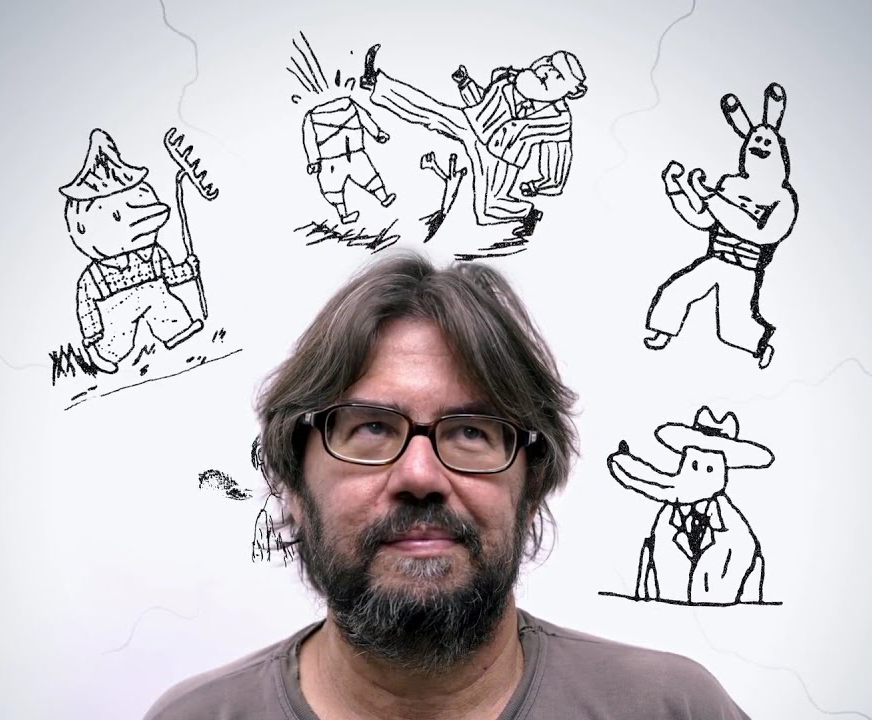
\includegraphics[width=\marginparwidth]{./images/PNLD2022-004-02.png}\\
O autor e ilustrador Fábio Zimbres (Arquivo pessoal)}


%313 caracteres
\paragraph{Publicações} Entre 1999 e 2001, desenhou a tirinha \textit{Vida boa}, publicada no jornal \textit{Folha de S.\,Paulo}. Em 2006, desenhou a história em quadrinho \textit{Música para Antropomorfos}, em parceria com a banda goiana Mechanics, republicada em 2018 pela editora Zarabatana. É criador e editor da Edições Tonto, cuja Coleção Mini Tonto publica livros de artistas alternativos brasileiros e latino-americanos.

%358 caracteres 
\paragraph{Currículo} Com a coleção Mini Tonto, ganhou o Troféu \textsc{hqm}ix de Projeto Gráfico em 1998. Em 2009, recebeu o prêmio Açorianos de Artes Visuais como Melhor Exposição Coletiva pela “Entre o Traço e o Espaço” e, um ano depois, foi indicado ao prêmio \textsc{pipa} (Prêmio Investidor Profissional de Arte). Em 2015, recebeu o prêmio Homenagem da Feira Miolo(s), realizada na Biblioteca Mario de Andrade. Um ano depois, em 2016, recebeu o \textsc{x} Prêmio Açorianos de Melhor Exposição Coletiva por “A Casa do Desenho”, no Museu do Trabalho, em Porto Alegre (\textsc{rs}).


\section{Sobre o gênero}

%55 caracteres
\paragraph{O gênero} O gênero deste livro é \textit{narrativa}. 

%596 caracteres
\paragraph{Descrição} Em sua base, pode-se definir a narrativa como um gênero que conta uma história, normalmente em estrutura linear, ou seja, começo, meio e fim, e com personagens. 
Dentre os tipos de narrativas mais comuns na literatura infantil, estão: mito, lenda, 
fábula e apólogo. Nos livros infantis, as possibilidades narrativas são quase ilimitadas, pois quase tudo pode integrar a narrativa e fazer parte dela como personagem, já que a capacidade reflexiva das crianças nesta idade ainda está em um nível primário. 

\Image{O gênero da narrativa proporciona ao leitor uma abertura ao mundo. (Pixabay/Tumisu; CC-BY-2.0)}{PNLD2022-004-07.png}

%603 caracteres
\paragraph{Interação} As narrativas são uma forma de inserir os sujeitos no mundo. 
São elas que apresentam boa parte dos valores culturais da sociedade 
onde se vive. Mas não é só passivo o papel das crianças nesta experiência. 
As interações entre dois ou mais personagens onde se verifica
uma ação de linguagem organiza e impulsiona experiências compartilhadas,
importantes para o desenvolvimento psíquico do sujeito nos primeiros anos de vida.
Neste sentido, as narrativas são uma ótima ferramenta para
apresentar o mundo e capacitar as crianças para viver nele, mas como se
trata de um trabalho com a linguagem, sempre dando espaço à individualidade, 
seja na compreensão das histórias, na identificação com as personagens, ou 
no ato de narrar.

%862 caracteres
\paragraph{Competências} 
Através de elementos dos mitos, contos e histórias do cotidiano (como é o caso desse livro), desenvolve-se a sensibilidade narrativa e a capacidade de imaginação das crianças. Para um bom desenvolvimento da capacidade narrativa e imaginativa é necessária a intermediação do educador, que vai trazer novos olhares, análises e discussões para ajudar a criança na construção do significado. Essas são etapas fundamentais para o desenvolvimento linguístico e a aquisição das competências de leitura e escrita. Por meio da narrativa, inclusive, a criança passa do diálogo ao monólogo, pois passa a ser capaz de elaborar um discurso para si com maior autonomia, sem a intermediação necessária no diálogo.
O conjunto de elementos verbais e visuais da narrativa proporcionam, assim,
uma abertura ao mundo e um convite para integrá-lo pela curiosidade e pela imaginação.


\section{Temas}

\subsection{Relacionamento pessoal e desenvolvimento de sentimentos de crianças nas escolas; nas famílias e nas comunidades (urbanas e rurais)}

%136 caracteres
\paragraph{Abordagem} O livro relaciona-se ao desenvolvimento das relações pessoais e dos sentimentos coletivos, uma vez que é focado na amizade entre as personagens e no companheirismo que desenvolvem em situações corriqueiras no meio de sua comunidade.

%206 caracteres
\paragraph{Descrição} O livro oferece uma ótima oportunidade de explorar 
e aprofundar os sentimentos de cuidado e solidariedade ao próximo, contribuindo para a inteligência emocional das crianças e a compreensão das dinâmicas das relações humanas.

%275 caracteres
\paragraph{Competências} Este tema relaciona-se, principalmente, ao 
campo da experiência O eu, o outro e o nós 
descrito pela \textsc{bncc}, que explora as relações interpessoais das crianças e sua capacidade de criar vínculos, percebendo as diferenças que constituem a sociedade e aprendendo a respeitá-las.


\section{Modelagem de aula}
A seguir você encontrará a descrição de uma aula modelo como exemplo 
prático de exploração do livro com estudantes. Esta seção apresentará 
orientações sobre como organizar a sala de aula para receber os 
estudantes, exercitar a interação verbal e prepará-los para o 
momento da leitura.

Em seguida, você encontrará a \textbf{Leitura dialogada}, um 
tópico destinado a te orientar para o momento específico da 
leitura com os estudantes. Por fim, no tópico 
\textbf{Propostas de atividades}, você encontrará ideias 
de práticas que pode explorar com as crianças em sala de 
aula antes, após e durante a leitura. 

Essas atividades podem ser trabalhadas de acordo com a 
disponibilidade do seu cronograma. Fique à vontade para adaptá-las 
da forma que achar melhor para os seus estudantes. Cada turma é única 
e o seu conhecimento prático das características de cada aluno será 
essencial para definir a melhor forma de aplicar essas ideias. 

O objetivo deste manual é oferecer algumas ideias 
e inspirações para um trabalho que pode ser desenvolvido tanto 
a curto, quanto a médio e longo prazo. Sinta-se à vontade para 
personalizar a aula e torná-la sua, aplicando seus conhecimentos, sua 
personalidade e aproveite para fortalecer 
seu vínculo com a turma.


\subsection{Antes de ler}

\BNCC{EI02EO01}
\BNCC{EI02EO03}
\BNCC{EI02EO04}
\BNCC{EI02EO05}
\BNCC{EI02EO07}
\BNCC{EI02CG05}

%Alterar o nível escolar nesse parágrafo.
Como este trabalho será realizado com crianças da \textbf{Creche 2}, 
que ainda não têm tanta intimidade com o livro enquanto objeto, você terá o 
papel essencial de mediar este contato. 

Nosso objetivo é que os próprios estudantes possam manusear 
e explorar o livro de forma autônoma, mas, para que isto aconteça, você 
pode ajudar a tornar o caminho mais convidativo com atividades que tenham 
intencionalidade educativa. 

A \textsc{bncc} define intencionalidade educativa como ``organização 
e proposição, pelo educador, de experiências que permitam às crianças 
conhecer a si e ao outro e de conhecer e compreender as relações com a 
natureza, com a cultura e com a produção científica, que se traduzem nas 
práticas de cuidados pessoais (alimentar-se, vestir-se, higienizar-se), 
nas brincadeiras, nas experimentações com materiais 
variados, na aproximação com a literatura e no encontro com as 
pessoas''.\footnote{\textsc{bncc}, página 39}

É importante manter essa intencionalidade em mente não apenas na condução 
das atividades propostas neste manual, mas também para aproveitar as 
oportunidades espontâneas de construir conhecimentos que podem surgir durante 
a interação direta com os estudantes.

\begin{enumerate}
%836 caracteres
\item \textbf{O ambiente}\quad Antes de iniciar o trabalho com o livro, é importante que você 
prepare o ambiente para receber a turma. Como o trabalho com o livro terá 
três momentos (antes, durante e depois da leitura), seria interessante que você 
criasse um ambiente para cada etapa. Nas \textbf{Sugestões de referências complementares} 
você encontrará um artigo que discorre sobre a importância da organização da sala 
de aula para a educação infantil, que pode ser um bom guia para a criação desses 
ambientes.
Para o momento antes da leitura, sugerimos uma atividade que explorar as características das crianças, observando suas relações de semelhança e diferença. É uma forma de introduzir a criança no assunto que será tratado na obra, além de estimular as competências relacionadas às interações sociais. Para isso, é interessante que as crianças se sentem em roda na sala de aula.

%413 caracteres
\item \textbf{Materiais}\quad Lápis de cor; folha sulfite A4. 

%632 caracteres
\item \textbf{Desenvolvimento}\quad Em roda, converse com as crianças a respeito das diferenças e semelhanças que existem dentro do grupo. Essas diferenças e semelhanças podem estar relacionadas à aparência física, à vestimenta, às preferências; diferenças de idade, de cidade ou bairro em que mora, ou de outras coisas observadas pelas crianças, percebidas pelo professor e que se julguem proveitosas. A proposta é que, a partir dessas observações, seja estimulado o reconhecimento do eu e do outro, além da coletividade que os integra. É possível que as crianças tenham dificuldades em ressaltar as características que surgem da relação com o colega. Sugere-se que a professora estimule a atenção aos detalhes que possam auxiliar na captação dessas diferenças. É importante que nessa conversa as crianças possam encontrar semelhanças entre os diferentes participantes do grupo, não se limitando ao colega mais próximo e, assim, espera-se que o professor faça essas observações no decorrer da ação. Em seguida, propõe-se que as crianças façam um desenho a respeito das suas características e das características de um colega da turma e compartilhem com o grupo.    

\item \textbf{Perguntas para avaliar}\quad A criança demonstra compreender que as diferenças existem? Há uma postura positiva em relação às diferenças dos colegas? A criança consegue expressar o que seu desenho representa? Consegue estabelecer relações de diferenças e semelhanças? 

\end{enumerate}


\subsubsection{A interação verbal} 
Criar situações em que as crianças precisam dialogar diretamente com 
você é uma das práticas mais importantes de Literacia, pois elas estimulam 
o desenvolvimento linguístico, ampliam o vocabulário e reforçam a 
capacidade dos estudantes de compreenderem o que ouvem e se expressarem 
pela fala. O diálogo livre com a criança também reforça sua autoestima, pois 
a faz se sentir ouvida e valorizada pelo adulto, ao vê-lo prestar atenção 
no que ela tem a dizer. Portanto, sempre que possível, reserve um tempo na 
aula apenas para a interação verbal. 

Como esse tipo de interação é espontânea e intimamente atrelada ao 
desenvolvimento de cada estudante, nossas orientações não serão específicas. 
A ideia é que você adapte este momento de acordo com as respostas e os 
repertórios das crianças. É um momento de estreitamento de vínculos e, portanto, 
fique à vontade para ser espontânea e para explorar os tópicos que achar 
mais interessantes para a sua turma.

Inicie as conversas com naturalidade, seguindo os objetos de atenção das crianças. 
Você pode partir de objetos que estejam analisando
para iniciar um assunto e incentivar que se expressem. Ainda que a
criança não fale corretamente, continue interagindo, 
pois a intenção aqui é que a criança perceba que outras pessoas estão respondendo 
à sua comunicação. 

Fique atento a todas as formas de expressão: os gestos, as falas, as 
expressões faciais, para onde olham\ldots{} tudo pode ser explorado durante a conversa. 
Demonstre curiosidade sobre eles, seja um ouvinte entusiasmado e incentive que eles 
conversem entre si. Faça perguntas e construa a resposta junto com as crianças. 

A seguir, algumas dicas que podem contribuir para que a interação verbal 
seja produtiva em sua sala de aula: 

\begin{enumerate}
\item Sente-se no chão e brinque com eles, estabelecendo 
contato visual. Além das pequenas frases que conseguem formar, vocalizações, 
gestos e expressões faciais podem ser boas formas de comunicar.

\item Não se esqueça que a conversa é uma troca e, portanto, 
evite ficar falando sozinho ou desvalorizar as respostas das 
crianças quando não conseguem formular frases completamente articuladas. 
Nunca descarte uma tentativa de comunicação. 

\item Evite utilizar falas negativas que desencorajam o diálogo. 
Se precisar que a turma 
corrija algum comportamento, explique claramente a razão e 
oriente com calma. Incentive positivamente as crianças e 
destaque o motivo de seus elogios. 

\item Aproveite alguns momentos durante a conversa para chamar 
a atenção das crianças para os sons das palavras e das letras que você 
acabou de usar ou que eles pronunciaram.  

\item Explore possibilidades de interação como apontar e 
nomear objetos, pessoas e animais, imitar a criança ou pedir que 
ela o imite, fazer caretas, reproduzir sons de 
animais para que repitam, ensinar os nomes de partes do corpo, 
entre outras atitudes que estimulem a comunicação com a criança. 

\item Muitas dessas dicas poderão ser aproveitadas pela 
família durante a prática da Literacia Familiar. Portanto, 
se achar necessário, compartilhe algumas destas orientações 
com as famílias dos estudantes.
\end{enumerate}


\subsection{A leitura dialogada}
Este é o momento em que será realizada a leitura propriamente dita. 
Se possível, crie um \textit{cantinho da leitura} em sua sala de aula. Um 
ambiente confortável, de preferência em que todos se sentem no chão ou 
em pufes para que consigam enxergar as ilustrações do livro que está 
sendo lido e interagir com facilidade. Se houver possibilidade, mantenha 
sempre os livros da turma em uma altura da estante que permita fácil 
acesso para os estudantes ou guarde os livros em uma caixa que as crianças 
possam mexer com autonomia. É importante que elas tenham autonomia para 
acessar os livros e se sintam à vontade para pegá-los sempre que quiserem. 

\Image{É importante que o cantinho da leitura proporcione autonomia para as crianças. (Tânia Rêgo/Agência Brasil; CC BY-NC 2.0)}{PNLD2022-004-08.png}

Outra possibilidade de ambiente para esta leitura, se a escola permitir, 
é efetuar essa leitura ao ar livre, embaixo de uma árvore, onde as crianças 
possam ouvir os sons dos pássaros e sentir o cheiro da grama. Sair da sala 
de aula pode oferecer um ótimo leque de experiências aos seus estudantes e 
reforçar a conexão entre os estudantes em diferentes ambientes.  

Reserve uma boa parte da aula para o momento da leitura com os estudantes, 
pois é importante que esse momento aconteça sem pressa. O objetivo da 
leitura dialogada é que seja uma leitura em bate-papo. A criança deve 
assumir um papel ativo na leitura, mesmo que ainda não seja capaz de 
ler sozinha. Além de promover o gosto pela leitura, esta prática estimula 
o desenvolvimento da linguagem, enriquece o vocabulário e 
aumenta o conhecimento de mundo.

%Especificar o livro.
No caso de \textit{Cada qual com seu gosto} o diálogo durante a leitura é 
ainda mais importante, considerando que as crianças ainda não têm domínio sobre o código escrito e, portanto, a compreensão do texto se apoiará principalmente na sua interação com elas. 
Você deve interagir com eles durante toda a 
leitura, fazendo perguntas e partindo de detalhes do livro para 
levantar novas questões. 

A seguir, algumas orientações para aproveitar este momento e desenvolver uma atividade durante a leitura: 

\begin{enumerate}
%177 caracteres
\item \textbf{Contexto}\quad Após a atividade anterior à leitura, as questões mobilizadas pelo livro ainda estarão frescas nas crianças, que brincaram e se divertiram em torno das diferenças e semelhanças entre elas. A partir do livro, propõe-se que seja ressaltada a questão das diferenças e de como elas podem (e devem) ser consideradas como positivas. Durante a leitura do livro, é importante ressaltar como cada personagem tem suas preferências e como elas são divertidas e fazem delas crianças únicas. Aconselha-se o professor a se sentar em roda com as crianças na sala de aula.

\item \textbf{Materiais}\quad Livro \textit{Cada qual com seu gosto}; se possível (não é imprescindível), um rádio ou outro aparelho de som.


\item \textbf{Desenvolvimento}\quad Esta atividade foi pensada para acompanhar a leitura do livro \textit{Cada qual com seu gosto}, aumentando a interação das crianças durante a leitura e sua compreensão da obra. É interessante que o professor leia previamente a obra, pensando em mais formas de explorar os personagens e suas características, enfatizando os aspectos positivos de cada um, além das sugestões aqui apresentadas.
A posição da turma em roda é necessária para que se crie um clima de acolhimento. 
 
%230 caracteres
\item \textbf{Manuseio}\quad Deixe que as crianças manuseiem o livro 
e explore com elas todos os elementos que o compõem. Mostre o que é a 
capa e onde estão as páginas.

%495 caracteres
\item \textbf{Diálogo}\quad Além de abordar as relações pessoais, presentes em qualquer sociedade, o livro aborda características das personagens comuns ao cotidiano: o gosto por frutas, por tomar sol, por ouvir histórias etc. Isso permite muitas pontes de diálogo com as crianças, que podem associar a história narrada às suas vidas. A atividade de pré-leitura já sugere esse diálogo durante a leitura, pois convida as crianças a expor suas opiniões e partilhar suas experiências que envolvem gostos e características próprias.

%346 caracteres
\item \textbf{Escuta}\quad Elogie atitudes positivas, como 
a boa interação com a história lida e a solicitação de interagirem com ela. Se os estudantes tentarem 
tomar o seu lugar e começar a falar sobre a história ou suas relações pessoais ou gostos próprios, valorize e escute com atenção o que estiverem falando. Mas não 
force a leitura. Se as crianças estiverem cansadas, faça outra atividade 
e retorne depois. 

\includepdf[nup=2x3, 				% grid
			%offset=-15mm -5mm, 	% posição
			scale=.8, 				% tamanho da página
            delta=4mm 4mm, 			
            frame,
            pages={5-6,15-16,39-40}]{./pdfs/\jobname_MIOLO.pdf}

%935 caracteres
\item \textbf{Leitura}\quad Enquanto lê, sugere-se que a professora mostre as figuras para as crianças e estimule que elas discutam sobre o que está sendo mostrado.
Faça perguntas como:

\begin{itemize}
\item Laura gosta de banana. Banana é um brinquedo?
\item O que é então uma banana?
\end{itemize}


Espera-se que as crianças digam comida ou fruta, e nesse momento pode-se questionar se alguma delas também gosta de banana ou prefere outra fruta, como maçã, limão, morango etc. É interessante que nesse momento as crianças possam falar sobre o que costumam comer em casa ou na escolinha.
Todos os personagens, e seus gostos, podem ser explorados através da leitura dialogada:

\begin{itemize}
\item Marcelo gosta de música. Quem aqui também gosta de música?
\item Qual música?
\item Cante um pedacinho?
\item Prefere dançar ou cantar?
\end{itemize}

Pode-se colocar uma música conhecida das crianças para que elas dancem em roda, reafirmando os vínculos comuns entre elas e criando um espaço de diversão e socialização que explora as ideias tratadas no livro. Caso não se tenha um rádio ou caixa de som, pode-se cantar com a turma.


Após esse momento, é interessante retornar ao livro, criando o vínculo entre a atividade lúdica e corporal e o momento de leitura. Assim, o hábito da leitura passa a estar associado a coisas dinâmicas e divertidas.

\Image{Durante a atividade musical com as crianças é interessante fazer uma roda para integrar a sala. (Jonas Banhos; CC BY-NC 2.0)}{PNLD2022-004-09.png}

%382 caracteres
\item \textbf{Interação}\quad Nomeie as ilustrações 
do livro, apontando para elas com o dedo e, ao mesmo tempo, reforçando sua ligação com a palavra que a representa. Destaque os sons de algumas 
palavras mais difíceis. Interrompa a leitura em alguns momentos e peça que 
os estudantes repitam palavras e sentenças do livro. Se possível, 
releia a mesma história outras vezes ou recrie narrativas em cima do livro, perguntando aos estudantes, por exemplo, o que eles gostariam de levar ao Zeca machucado; ou com quem eles gostariam de estar ao lado em situações semelhantes.

\item \textbf{Perguntas para avaliar}\quad As crianças demonstram reconhecer a diferença como algo positivo? As crianças diferenciam suas características das outras dos colegas e familiares? As crianças conseguem estabelecer relação de generalização, como o grupo das frutas (banana, maçã, limão), o grupo das artes (música, dança, teatro), grupo das brincadeiras (roda-roda, amarelinha, pular corda)? 
\end{enumerate}


\subsection{Propostas de atividades}

\BNCC{EI02EO03}
\BNCC{EI02EO04}
\BNCC{EI02EO05}
\BNCC{EI02CG05}
\BNCC{EI02EF01}


\begin{enumerate}
%700 caracteres
\item \textbf{Contexto}\quad Esta atividade propõe que as crianças possam reconhecer o colega e uma ou mais características que possam perceber nele. O objetivo é que, ao evidenciar a característica do outro, seja possível adotar uma posição acolhedora e positiva em relação às diferenças.

\item \textbf{Materiais}\quad Lápis de cor; giz de cera; folha sulfite A4.

%650 caracteres
\item \textbf{O ambiente}\quad Sala com mesa e cadeira.

\Image{Em duplas, as crianças vão desenhar umas às outras, percebendo diferenças e semelhanças. (Prefeitura Municipal de Itanhaém; CC-BY-2.0)}{PNLD2022-004-10.png}

%950 caracteres
\item \textbf{A atividade}\quad Forme duplas entre as crianças e peça que elas observem as características do colega com quem forma dupla. Uma a uma, peça que falem sobre uma ou mais características de seu colega que observaram. A dupla irá dizer para a turma o que considera legal ou bonito no colega. Após todas as crianças falarem, a proposta é que possam desenhar seu colega, evidenciando essas características boas que foram comentadas anteriormente na roda de conversa. É possível que as crianças tenham alguma dificuldade em se expressar por conta da idade, então é importante que a professora estimule a criatividade e a percepção das crianças, dando exemplos que possam ajudar as mesmas a reconhecer essas características, tais como:

\begin{itemize}
\item Camila usa tranças;
\item Pedro usa óculos;
\item Daniela gosta de bonecas.
\item João veste azul
\end{itemize}

Com essa dinâmica, as crianças vão aprofundando a percepção sobre as diferenças ao seu redor, aprendendo a verbalizá-las e expressar-se de forma respeitosa acerca da pluralidade de gostos, opiniões e corpos que constituem seu entorno em sociedade. 

%550 caracteres
\item \textbf{Interação}\quad A estrutura da atividade é toda baseada na interação entre as crianças, o professor e a história do livro. Após a dinâmica, o professor pode retornar ao livro para que as crianças o manuseiem. Observe o comportamento dos alunos, se eles mudaram de opiniões após as brincadeiras ou se apresentam outra percepção sobre as diferenças e características das personagens. Incentive que eles tentem repetir algum trecho da história,
faça perguntas e proponha que imaginem juntos do que as personagens devem gostar, além do que está expresso no livro. Quando as crianças propuserem suas ideias, interaja com o pensado e apresentado pelas crianças, fazendo perguntas que as auxiliem a desenvolver o pensamento iniciado.

\item \textbf{Perguntas para avaliar}\quad A criança consegue perceber a diferença entre seus colegas? A criança se expressa verbalmente sobre essas diferenças? A criança precisou de mais estímulo do que o esperado para se expressar?
\end{enumerate}


\section{Literacia familiar}
O \textsc{pna} dá destaque especial para a importância do envolvimento da família 
no processo pedagógico nesta faixa etária e denomina Literacia Familiar o conjunto 
de experiências e práticas relacionadas à linguagem (oral, escrita ou lida) vivenciadas 
com os cuidadores. 

Essas estratégias podem começar a ser colocadas em prática desde a 
gestação e continuar até o final da adolescência. São práticas simples e divertidas 
que estimulam o desenvolvimento de quatro atividades fundamentais: ouvir, falar, 
ler e escrever que criam momentos de afeto e interação para a família. 

Para que esse trabalho conjunto entre escola e família funcione, é 
fundamental que a escola esteja em constante diálogo com os responsáveis e 
você consiga orientá-los. Um grupo em aplicativos de mensagens instantâneas ou um 
grupo de e-mails são saídas viáveis para que a comunicação se estabeleça e pode ser 
uma forma útil das famílias compartilharem suas vivências e trocarem sugestões 
de abordagens, sempre contando com a sua mediação. 

Com o objetivo de incentivar 
a prática da \textit{literacia familiar}, se possível, organize um rodízio entre os familiares 
das crianças para emprestar o livro da biblioteca da turma. Neste caso, crie um caderno 
de registro e estabeleça períodos para cada família ficar com o livro. É importante 
que os familiares compreendam a seriedade deste compromisso, pois o livro pertence 
ao acervo da sala e, portanto, deve ser bem cuidado e devolvido na data acordada. 

Se não for possível garantir o acesso direto dos cuidadores da criança ao livro, 
grave um vídeo direcionado a eles, contando a história e apresentando algumas 
das ilustrações. O importante é que os familiares saibam com clareza qual livro 
está sendo trabalhado, a história contada e se sinta seguro para explorar as temáticas 
do livro com a criança. Orientações claras e a manutenção do canal de comunicação com 
os responsáveis é essencial para que eles se sintam seguros e à vontade para fazer perguntas 
se tiverem dúvidas. 

Neste manual, você encontrará algumas práticas que podem ser 
recomendadas aos familiares para ajudá-los a expandir e aprofundar o trabalho 
que você iniciou em sala de aula.


\subsection{Importância da leitura}
Na escola, aprendemos a ler letras, mas é importante ter em mente que nós 
lemos o mundo desde muito pequenos: “lemos” os animais que passam pelos nossos 
quintais, a expressão no rosto dos nossos familiares, as cores que pintam o céu 
em um fim de tarde. 

Vamos aprendendo, ao longo da vida, a interpretar acontecimentos 
e sons que escutamos e a utilizá-los para nossa comunicação. Aprender a ler textos e 
escrevê-los expande a nossa leitura do mundo, pois permite que sejamos capazes de 
interpretar um código e experimentar, a partir dele, novas experiências e conhecimentos. 

O simples contato com os livros já permite um leque grande de sensações: 
sentimos as texturas, as formas, vemos as cores do livro, escutamos o som da página 
virando e o som da voz do narrador, se a história estiver sendo lida em voz alta. Para uma 
criança pequena, são experiências que podem contribuir diretamente com o desenvolvimento psicomotor 
e cognitivo. 

Nosso papel, enquanto mediadores de leitura, é contribuir para que essas 
sensações sejam associadas a momentos positivos, de construção de 
conhecimento e exercício de imaginação. 

Com os livros, podemos conhecer mais da história humana, descobrir informações 
novas sobre sociedades diferentes da nossa, imaginar situações e contextos inéditos 
para nós e aumentar o nosso repertório. São por meio deles que melhoramos nossa 
capacidade de interpretação, de expressão, de análise e senso crítico. Boas habilidades 
leitoras podem contribuir para o desenvolvimento de um estudante em todas as outras 
disciplinas, pois exercem influência direta na forma como absorvemos e 
construímos conhecimento.


\subsection{O papel da família na formação do leitor}
A família é peça fundamental na formação do leitor, pois é ela quem primeiro 
ensina a criança a ler. Não apenas os textos escritos, mas a ler o mundo, a 
interpretar os estímulos que a cercam, a construir seu próprio vocabulário e a 
comunicar seus pensamentos e necessidades.

O universo das letras é muito presente na vida das crianças antes mesmo de sua 
entrada na escola. Aparece nas histórias e ilustrações do livro que o cuidador 
lê ao colocá-la para dormir, nas situações em que vê os responsáveis se comunicarem 
pela escrita ou nos textos que podem permear seu cotidiano (nos outdoors, na 
televisão, no celular, manuais de instrução entre outros). 

Os familiares têm, 
portanto, uma ótima oportunidade de apresentar a leitura com leveza, de forma 
prazerosa, associado ao contexto em que a criança vive e à momentos de diversão. 
Você poderá orientar os pais nesta tarefa, ensinando-os com este guia a aproveitar 
as oportunidades para trabalhar a Literacia com a criança.


\subsubsection{Práticas de literacia familiar} 

São muitas as experiências que a prática da \textit{literacia familiar} 
pode oferecer às crianças. A seguir, explicamos cada uma delas para que você possa, 
se achar necessário, compartilhar com os responsáveis enquanto estiver orientando-os: 

\paragraph{Interação verbal} Aumentar a quantidade de conversas com as 
crianças, fazendo perguntas para incentivar o diálogo.

\paragraph{Leitura dialogada} Interagir com a criança durante a leitura 
em voz alta, criar expectativa sobre o livro, chamar a atenção para detalhes 
das ilustrações e comentar o enredo.

\paragraph{Narração de histórias} Interagir com a criança enquanto 
estiver narrando uma história, por exemplo, incluindo-a na ação, utilizando 
marionetes ou permitindo que ela complete a narrativa.

\paragraph{Contatos com a escrita} Apresentar as letras para as 
crianças, incentivar que tentem escrever ou ler, ajudá-los a desenhar letras, 
entre outras formas de incentivar o contato com as palavras.

\paragraph{Atividades diversas} Qualquer atividade com a criança 
pode ser utilizada para contribuir para a alfabetização. Jogos, brincadeiras, 
instrumentos musicais, canto, dança, passeios e viagens oferecem boas 
oportunidades de aprendizado.

\paragraph{Motivação} Atitudes que motivem as crianças à envolver-se com 
o mundo da leitura e da escrita.

\subsection{Exercitando a literacia familiar}

\BNCC{EI02EO02} 
\BNCC{EI02EO03} 
\BNCC{EI02EO04} 
\BNCC{EI02EO05} 
\BNCC{EI02CG05} 
\BNCC{EI02EF01}
\BNCC{EI02EF03}

\begin{enumerate}
%700 caracteres
\item \textbf{Como começar}\quad O contato da família com a criança e o livro começam desde a primeira atividade proposta. Peça que os familiares conversem com as crianças a respeito das características que possuem, tais como idade, gênero, atividades principais.
O familiar pode ressaltar as diferenças entre ele e a criança. Por exemplo: Joana tem 3 anos e Márcia, sua mãe, tem 32; Joana vai à escolinha e Márcia trabalha como garçonete.
Fale sobre essas diferenças e as evidencie. A criança, assim, começa a perceber a relação com o Outro no seio da própria família. As crianças, com ajuda dos pais, podem fazer um desenho que represente essas diferenças na sua família e trazer para a sala de aula, socializando com os colegas.
Essa é uma forma de iniciar o contato dos pais com as crianças na leitura, pois os envolve nas atividades e competências que serão desenvolvidas em sala de aula.

%650 caracteres
\item \textbf{Leitura}\quad 

 

A família pode continuar 
explorando os temas apresentados pelo livro. Uma das formas de fazer isso é solicitar aos pais que ajudem a criança a eleger um objeto que gostem para levar e mostrar para a turma.
Nesse diálogo, os pais podem explorar os gostos da criança, perguntar sobre o gosto de seus colegas de turma e as diferenças que observam entre eles. Os pais podem relacionar esses gostos e suas diferenças com o livro lido em sala: mostrando as semelhanças entre as personagens e as crianças, que também são constituídas pelas mais diversas características.
Ao levar um objeto de preferência para a classe, a criança também está trazendo seu universo pessoal para o grupo. Isso é importante para estreitar o vínculo entre eles e, também, com os pais, que participaram dessa escolha e ajudaram a criança a desenvolver sua ideia.
Outra possibilidade, quando a família tem acesso ao livro, é ler alguns trechos com a criança em um horário estipulado para isso. A leitura em família é importante pois relaciona o ato de ler e manusear um livro com o campo de suas experiências afetivas.

%1073 caracteres
\item \textbf{Instrução}\quad Informe aos pais sobre a estrutura do livro e as principais competências desenvolvidas em sala de aula.
Oriente-os a, quando possível, ler alguns trechos da história com a criança, confabulando sobre suas próprias experiências com as diferenças, recorrendo a exemplos de amigos, familiares, no trabalho etc.
Os familiares também podem incentivar a percepção sobre diferenças e semelhanças no cotidiano da criança, estabelecendo as relações de generalização, tais como: boneca, carrinho, massinha = brinquedos; camiseta, sapato, vestido = roupas; arroz, batata, leite = alimentos/comida.  
Desta forma, as crianças vão relacionando as experiências de semelhança e distinção do livro ao seu cotidiano.
Ademais, quando os responsáveis leem com as crianças, colocam-na em contato com duas experiências de leitura distintas: através da mediação em sala de aula e em família. 
Mesmo pequenas, as crianças conseguem perceber a diferença entre 
as formas de contar, e elementos da narração em casa podem ajudá-la a compreender 
sentidos e perceber detalhes que não foram explorados em sala de aula. Se possível, depois da leitura, oriente 
que voltem ao livro e tentem identificar as personagens e os gostos que as caracterizam.

Outra opção é entregar o livro para a criança e pedir que ela tente se lembrar
do que foi falado em sala de aula, quais elementos foram destacados e enfatizados pelo educador e pelos colegas. Pode-se orientar os pais a pedir que a criança conte sobre as atividades realizadas em sala, tentando se lembrar dos gostos e diferenças dos seus coleguinhas, pois isso estimula a criatividade e a memória dos alunos. Mesmo que a memória não pareça 
completa para o adulto, é importante que ele ouça com atenção e 
valorize todas as tentativas da criança. Afinal, ao tentar recontar, 
ela manipulará o livro, treinará a coordenação motora, conhecerá as texturas 
do objeto e poderá imitar a forma como o adulto 
conta a história, treinando a fala. 
\end{enumerate}

 
\section{Sugestões de referências complementares}

\subsection{Livros} 

\begin{itemize}
\item \textsc{lins}, Guto. \textit{Livro infantil? projeto gráfico, metodologia, subjetividade}. São Paulo: Rosari, 2002.

Livro que aborda a importância das escolhas visuais (ilustração, projeto gráfico, lettering) na literatura infantil.  

\item \textsc{hunt}, Peter. \textit{Crítica, teoria e literatura infantil}. São Paulo: Cosac Naify, 2010.

Livro sobre crítica de literatura infantil que contêm definições de livro ilustrado e livro imagem. 
\end{itemize}

\subsection{Artigos}

\begin{itemize}
\item \textsc{sardelich}, Maria Emilia. Leitura de Imagens, Cultura Visual e Prática Educativa. 
In: Cadernos de Pesquisa. V.36, n.128, p.451-472, mai/ago.2006. Disponível em: \url{https://www.scielo.br/pdf/cp/v36n128/v36n128a09}. 
Acesso em 29 abr 2021. 

Artigo acadêmico que discorre sobre a importância de trabalhar cultura 
visual na educação na sociedade contemporânea. 

\item \textsc{pranke}, Marha Elfrida. Organização dos espaços da sala de aula na Educação Infantil. Disponível em: \url{http://centraldeinteligenciaacademica.blogspot.com/2016/04/organizacao-dos-espacos-da-sala-de-aula.html}. Acesso em 04 mai 2021. 

Artigo acadêmico que discorre sobre a importância da rotina e de criar ambientes dentro da sala de aula na Educação Infantil.  
\end{itemize}

\subsection{\textit{Sites}}

\begin{itemize}
\item Vídeos “Conta pra mim” no site do PNA. Disponível em: \url{http://alfabetizacao.mec.gov.br/contapramim}. 
Acesso em 13 abr. de 2021.

Página do \textsc{mec} com vídeos sobre leitura dialogada que visam incentivar a Literacia Familiar. Muitas das 
técnicas, explicações e materiais disponíveis nessa página podem ser utilizados em aula, mas o site também 
pode ser uma ótima indicação para ajudar a direcionar os cuidadores dos estudantes a praticar 
a literacia familiar e leitura dialogada.

\item Vídeo “Livros de imagem: como utilizar com as crianças?” do canal Conta Outra. Disponível em Youtube. 
Acesso em 14 abr. 2021. 

Neste vídeo, a pedagoga Bel explica o que são livros de imagem e faz sugestões para mediar a leitura com 
crianças. Se você achar conveniente, esse vídeo pode ser recomendado aos familiares da criança 
para inspirá-los na leitura dialogada. 
\end{itemize}

\section{Bibliografia comentada}

\subsection{Livros}

\begin{itemize}
\item \textsc{brasil}. Ministério da Educação. Base Nacional Comum Curricular. Brasília, 2018.

Consultar a \textsc{bncc} é essencial para criar atividades para a turma. Além de especificar 
quais habilidades precisam ser desenvolvidas em cada ano, é fonte de informações sobre 
o processo de aprendizagem infantil. 

\item \textsc{brasil}. Ministério da Educação. Secretaria de Alfabetização. Conta pra mim: Guia de Literacia Familiar. 
Brasília: \textsc{mec, sealf}, 2019. Disponível em: \url{http://alfabetizacao.mec.gov.br/images/conta-pra-mim/conta-pra-mim-literacia.pdf}.

Este guia é voltado aos pais e oferece explicações em uma linguagem bastante acessível e detalhada as práticas de Literacia Familiar, 
como praticar leitura dialogada, como narrar histórias, como exercitar interação oral, formas de proporcionar contatos com a escrita à criança etc. 
 
\item \textsc{brasil}. Ministério da Educação. Secretaria de Alfabetização. PNA Política Nacional de Alfabetização/Secretaria 
de Alfabetização. Brasília: \textsc{mec, sealf}, 2019.

Um guia fundamental para trabalhar pré-alfabetização e alfabetização de estudantes, que ressalta a importância da Literacia e da Numeracia. 

\item \textsc{van der linden}, Sophie. Para ler o livro ilustrado. São Paulo: Cosac Naify, 2011.

Livro sobre as particularidades do livro ilustrado, que apresenta as diferenças entre o livro ilustrado e o livro com ilustração. 
\end{itemize}

\subsection{Artigos}

\begin{itemize}
\item \textsc{costa}, A. C. C.; \textsc{santos neto}, J. A.; \textsc{bortolin}, S; \textsc{pereira}, Ana Paula. O livro de imagem e a mediação na escola. 
In \textsc{vii secin}, Universidade de Londrina. Disponível em \url{http://www.uel.br/eventos/cinf/index.php/secin2017/secin2107/paper/viewFile/445/296}. 
Acesso em 29 abr 2021
. 
Esse artigo reflete sobre a importância de se apresentar livros de imagem para os estudantes na escola para que as crianças aprendam a ler imagens. 

\item \textsc{nannini}, P. B. R.; \textsc{medeiros}, J. P. S.; \textsc{ribeiro}, J. M. Leitura em cena: Vivências em sala de aula com livro de imagens. 
Literartes, n. 3, p. 82-101, 2014. DOI: 10.11606/issn.2316-9826.literartes.2014.89204. 
Disponível em \url{https://www.revistas.usp.br/literartes/article/view/89204/92115}. Acesso em 29 abr. 2021. 

Artigo acadêmico sobre um trabalho utilizando o mesmo livro de imagem com crianças da educação infantil e ensino médio. 
É uma forma interessante de perceber que a leitura de imagens pode ser explorada com qualquer faixa etária. 
\end{itemize}

% 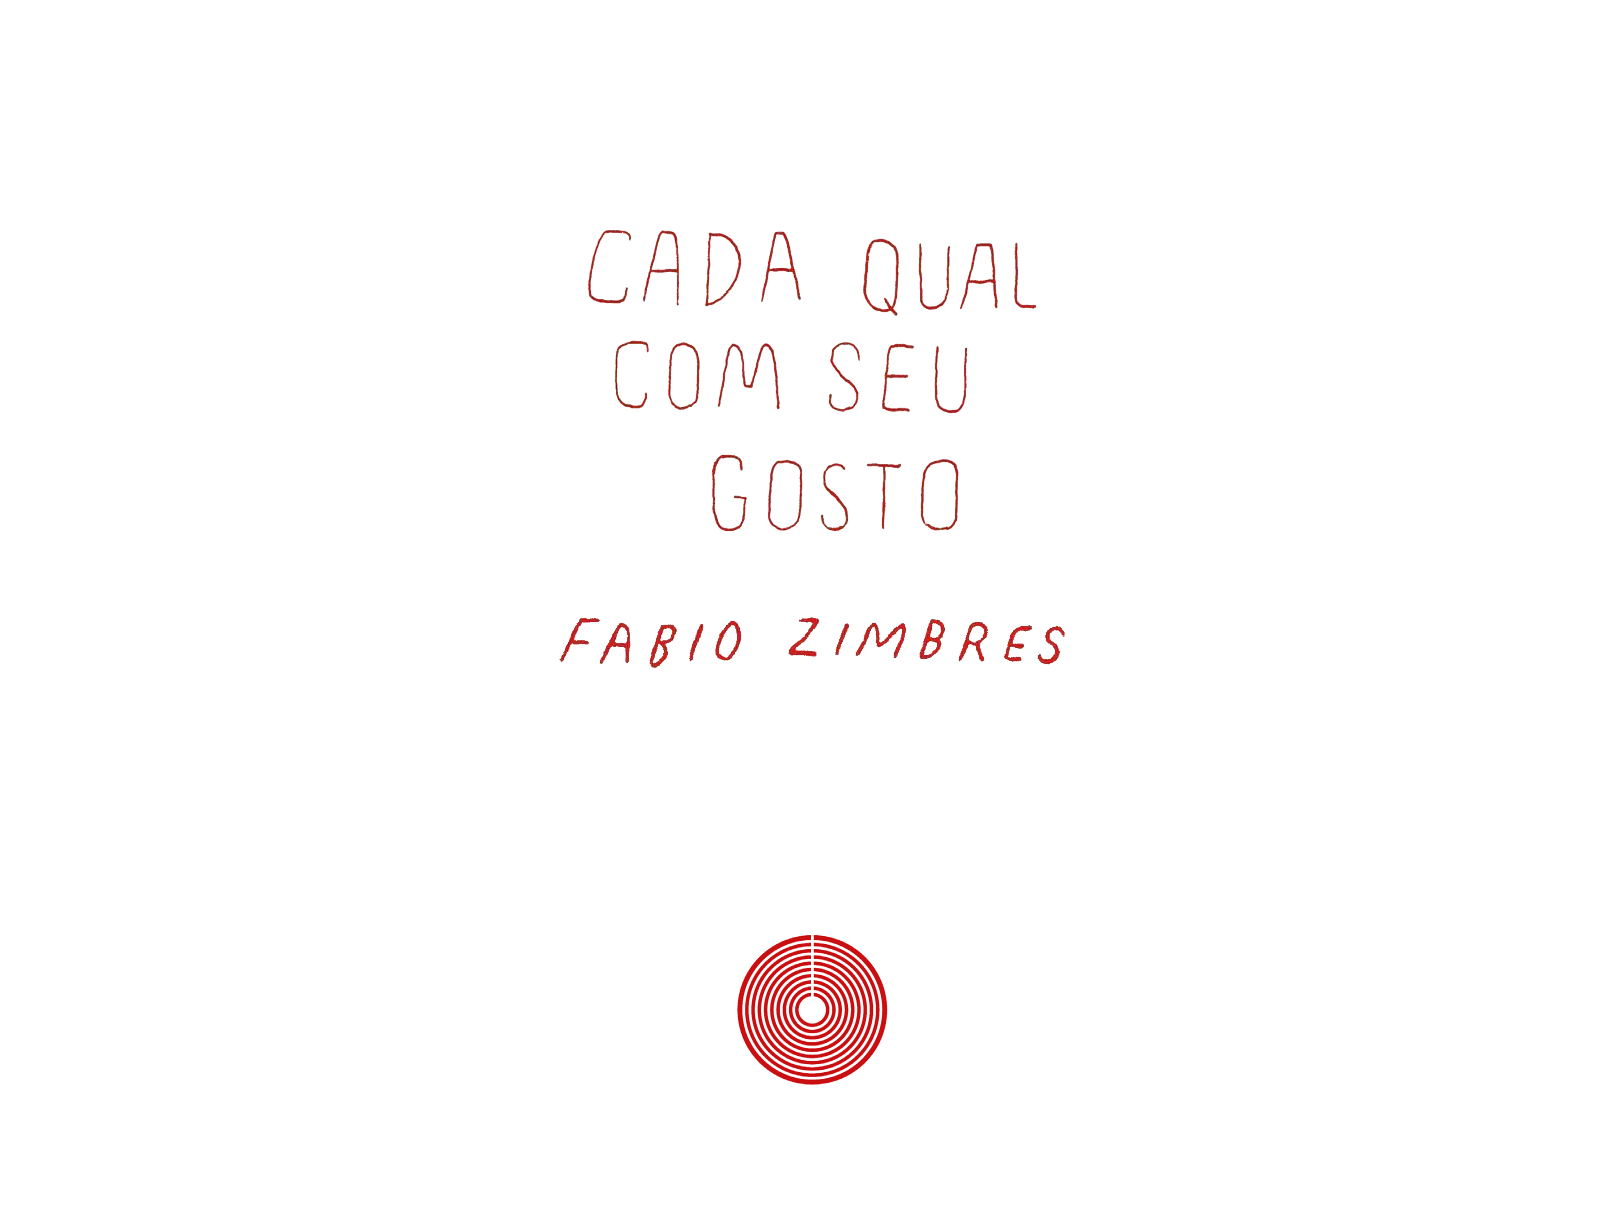
\includepdf[nup=2x2, 					% grid
			% offset=-15mm -5mm, 		% posição
			% scale=.8, 				% tamanho da página
            % delta=4mm 4mm, 			
            % frame,
            % pages={1-4}]{pdfs/PNLD2022-004_MIOLO.pdf}

\end{document}
